\chapter{نصب اوبونتو}
\section{دانلود و آماده‌سازی اولیه}
در این قسمت، شما با توجه به مشخصات سیستم خود، بین نسخه ۳۲ بیتی و ۶۴ بیتی نسخهٔ مناسب با معماری کامپیوترتان را از \href{http://www.ubuntu.com/download/desktop}{وب‌گاه اوبونتو} دانلود می‌کنید و بعد از اتمام دانلود، ۲ روش برای نصب دارید: نصب با \lr{DVD} یا نصب با \lr{USB}.

\subsection[نحوهٔ رایت روی DVD]{نحوهٔ رایت روی \lr{DVD}}
بعد از دانلود \lr{ISO}ی مناسب، آن را روی یک دیسک نوری خام بنویسید. سیستم عامل‌های مختلف، ابزارهای متفاوتی برای این کار دارند.

\subsubsection{در ویندوز}
در ویندوز می‌توان از \lr{InfraRecorder}، \lr{Clone CD} یا \lr{Nero} استفاده کرد.

\subsubsection{در \lr{Mac OS X}}
این سیستم عامل به صورت پیش‌فرض ابزار \lr{Disk Utility} را دارد که در مسیر:\\
\begin{flushleft}
\lr{Applications -> Utilities -> Disk Utility}\\
\end{flushleft}
قابل دسترس است. ابزار \lr{Disk Utility} را اجرا و \lr{ISO} را به قاب سمت چپ بکشید. بعد از زدن تیک \lr{Verify burned data}، روی \lr{Burn} کلیک کنید.

\subsubsection{در گنو/لینوکس}
کاربران گنو/لینوکس نیز می‌توانند از \lr{Brasero} یا \lr{K3b} استفاده کنند.

\subsection[نحوهٔ نصب بر روی USB]{نحوهٔ نصب بر روی \lr{USB}}
\subsubsection{در ویندوز}
می‌توان از \lr{Pen Drive Linux} یا \lr{LiLi} استفاده کرد. کار با این ابزارها بسیار ساده است. نوع توزیع (اوبونتو) و محل فایل \lr{ISO} دانلود شده را به نرم‌افزار بدهید و درایو حافظهٔ فلش را مشخص کنید.

\subsubsection{در \lr{Mac OS X}}
به کاربران \lr{OS X} توصیه می‌شود که از \lr{CD} یا \lr{DVD} استفاده کنند. زیرا رایانهٔ \lr{OS X} آن‌ها، قابلیت راه‌اندازی از طریق فایل‌های \lr{ISO} را ندارد.

\subsubsection{در گنو/لینوکس}
می‌توان از \lr{Unebootin} (روی تمام توزیع‌ها) و یا \lr{Ubuntu Startup Disk Creator} (مخصوص اوبونتو) استفاده کرد.


\section{نصب و راه‌اندازی}
بعد از ریختن اوبونتو روی \lr{DVD} یا \lr{USB}، باید آن را بوت کنید. برای بوت کردن از راه دی‌وی‌دی یا یواس‌بی، باید به دفترچهٔ مادربورد رایانه‌تان مراجعه کنید یا در اینترنت جست‌وجو کنید.\\
بعد از اینکه رایانه را با اوبونتو بوت کردید، دو انتخاب پیش‌رو دارید: انتخاب اول، نصب اوبونتو و انتخاب دوم، امتحان‌کردن اوبونتو است. با انتخاب گزینهٔ دوم، شما در هر زمان که تمایل به نصب داشتید، می‌توانید با کلیک بر روی آیکون نصب اوبونتو، آن را نصب کنید.\\
\begin{center}
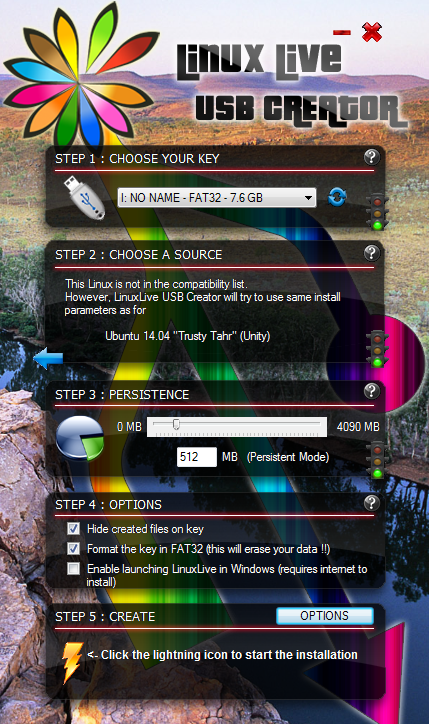
\includegraphics[scale=0.45]{pics/1.jpg}\\
\end{center}
در بخش بعد اوبونتو به شما چند انتخاب می‌دهد.
\begin{description}
\item[انتخاب اول]: نصب اوبونتو در کنار سیستم عامل فعلی\\
اگر دستگاه شما به اندازهٔ کافی (حداقل ۸ گیگابایت) فضای خالی داشته باشد، این گزینه برای شما نمایش داده می‌شود و اوبونتو به میزان دلخواه خودش، بخشی از فضای خالی روی هارد شما را به خودش اختصاص می دهد.

\item[انتخاب دوم]: پاک کردن سیستم عامل فعلی و نصب اوبونتو به جای آن\\
اگر دیگر تمایلی به استفاده از سیستم عامل فعلی خودتان ندارید، می‌توانید با انتخاب این گزینه، اوبونتو را به جای آن جایگزین کنید. توجه داشته باشید که در صورت انتخاب این گزینه، تمام اطلاعات شما پاک خواهد شد.

\item[انتخاب سوم]: تنظیمات دستی (\lr{Something Else})\\
در این قسمت شما می‌توانید تنظمات دلخواه خودتان را داشته باشید؛ مثلا یکی از پارتیشن‌های خود را پاک کرده و به اوبونتو اختصاص دهید.\\
\begin{center}
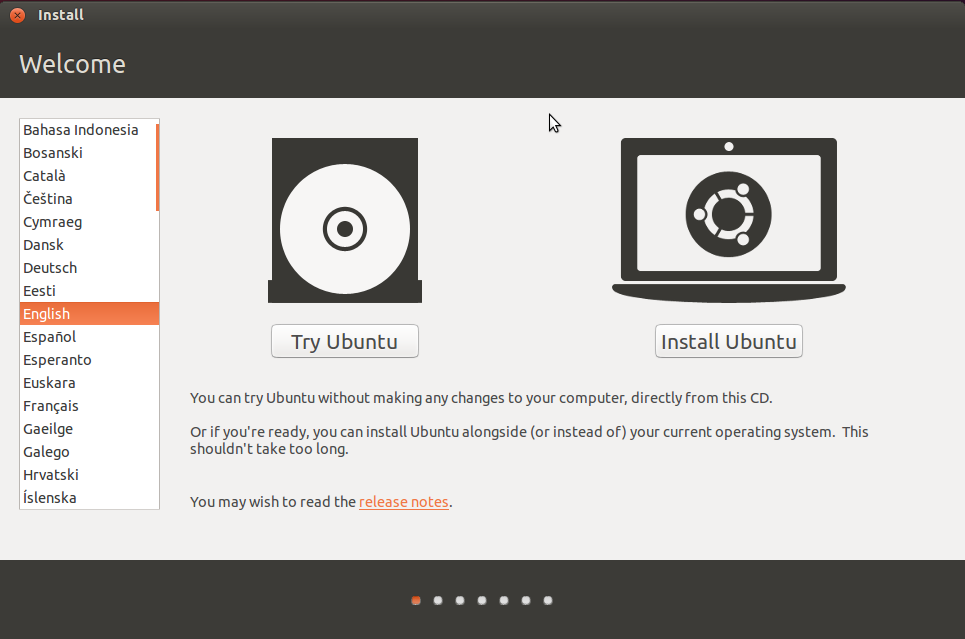
\includegraphics[scale=0.45]{pics/3.jpg}\\
\end{center}
* اگر فضای خالی و تمایلی به پاک‌کردن یکی  از پارتیشن‌هایتان ندارید، می‌توانید از نصب خارج شده و در بخش امتحان زنده اوبونتو، با برنامه \lr{GParted} بخشی از فضای خالی پارتیشن  دلخواه خود را انتخاب کنید و آن را از پارتیشن جدا کنید و یا این‌که این کار را با برنامه‌های مخصوص کار با پارتیشن‌ها در سیستم عامل فعلی‌تان انجام دهید.
\end{description}

اوبونتو به حداقل ۲ پارتیشن احتیاج دارد: اولی پارتیشن اصلی و دیگری پارتیشنی برای حافظهٔ مجازی.\\
برای اضافه‌کردن حافظهٔ مجازی، شما باید روی \lr{+} (\lr{Add}) کلیک کنید و در بخش نوع پارتیشن (\lr{Type for the new partition})، گزینه \lr{Logical} را انتخاب کنید. در بخش \lr{New partition size in megabytes} هم میزان فضایی تقریبا برابر با رم دستگاه یا کمی بیش‌تر را بدهید و در بخش \lr{Use as}، گزینهٔ \lr{swap area} را انتخاب کنید. \lr{OK} را بزنید.\\
برای اضافه‌کردن پارتیشن بعدی، روی فضای خالی باقی‌مانده کلیک کنید و \lr{+} (\lr{Add}) را بزنید. در بخش نوع پارتیشن \lr{Primary} و در بخش \lr{Use as}، ترجیحاً \lr{Ext4} را انتخاب کنید. در قسمت \lr{Mount point} هم گزینه \lr{/} را برگزینید.\\
پس از انجام این کارها، روی گزینهٔ \lr{Install Now} کلیک کنید تا اوبونتو شروع به نصب‌شدن کند.\\
در بخش بعد، روی محل زندگی خود در نقشه کلیک کنید تا زمان کامپیوتر را تنظیم کنید.\\
\begin{center}
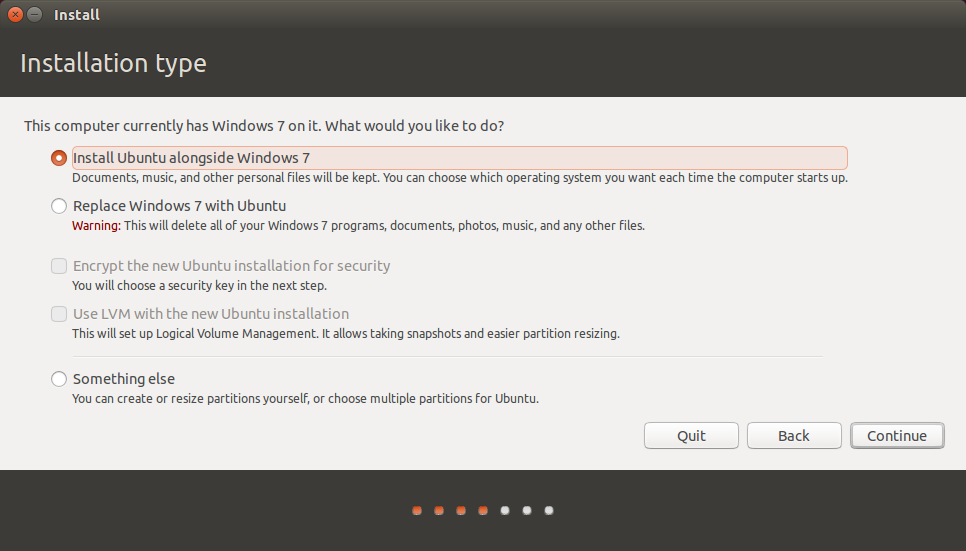
\includegraphics[scale=0.41]{pics/6.jpg}\\
\end{center}
در بخش بعد زبان \lr{Persian} را انتخاب کنید و روی ادامه (\lr{Continue}) کلیک کنید.\\
\begin{center}
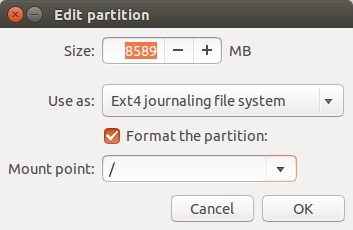
\includegraphics[scale=0.41]{pics/7.jpg}\\
\end{center}
در این قسمت مشخصات کاربری خود، همراه با گذرواژه را وارد کنید.
\begin{center}
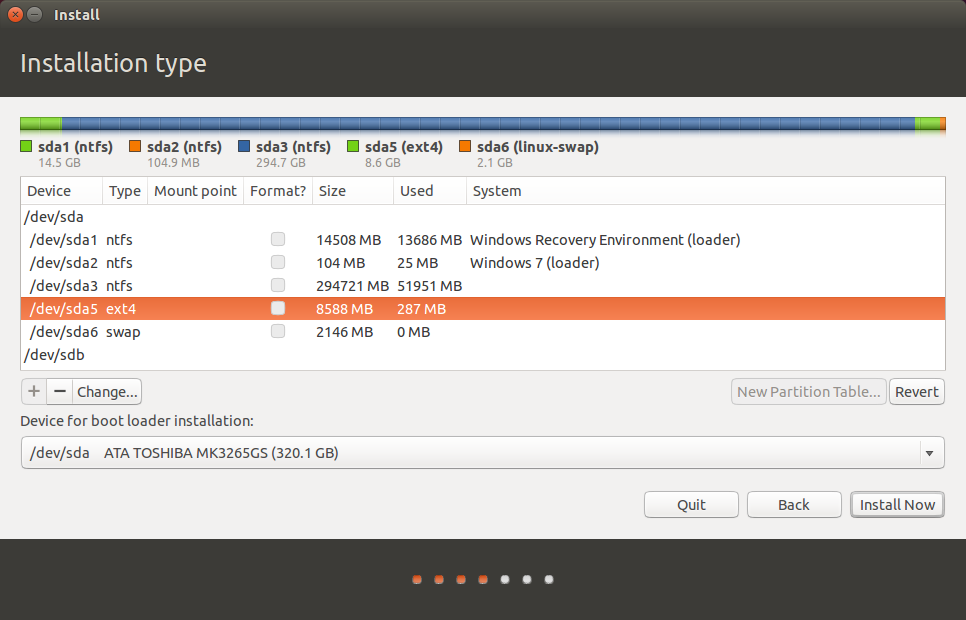
\includegraphics[scale=0.43]{pics/8.jpg}
\end{center}
در مرحلهٔ بعدی در صورتی که حساب \lr{Ubuntu One} داشته و به اینترنت وصل باشید، می‌توانید اطلاعات حساب را وارد کنید تا پرونده‌ها و اطلاعات‌تان همگام‌سازی شود.
\begin{center}
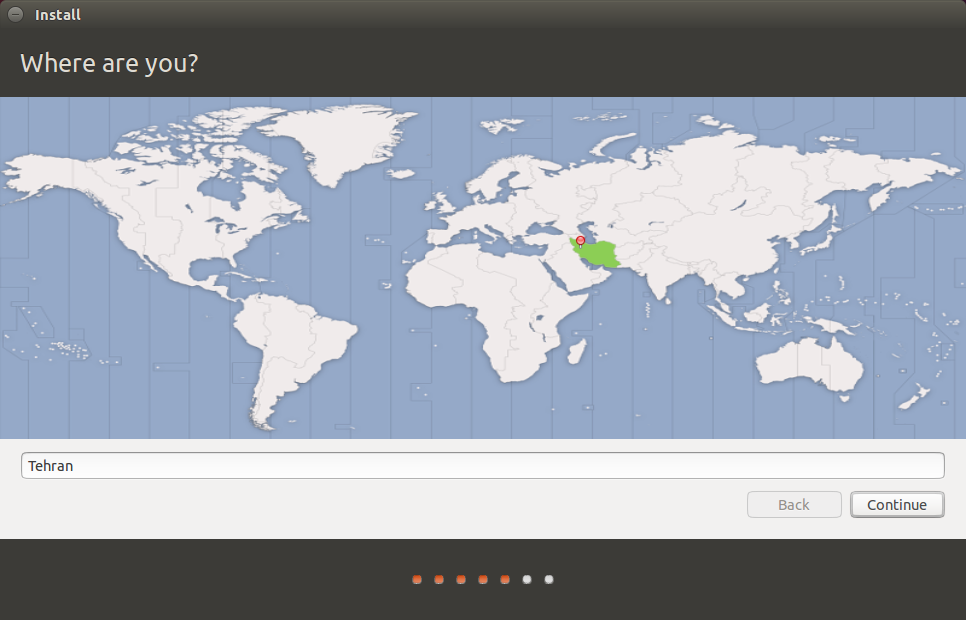
\includegraphics[scale=0.43]{pics/9.jpg}
\end{center}
اوبونتو خیلی سریع نصب خواهد شد. شما می‌توانید در این فرصت توضیحات مربوط به اوبونتو را مطالعه کنید تا نصب تمام شود.
\begin{center}
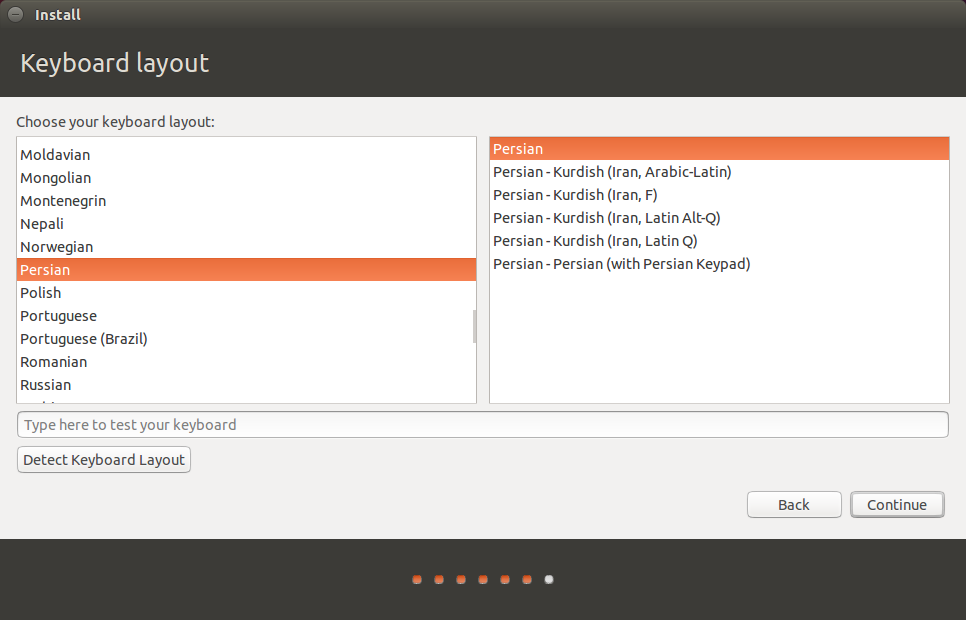
\includegraphics[scale=0.45]{pics/10.jpg}
\end{center}
